% This is samplepaper.tex, a sample chapter demonstrating the
% LLNCS macro package for Springer Computer Science proceedings;
% Version 2.21 of 2022/01/12
%
\documentclass[runningheads]{llncs}
%
\usepackage[T1]{fontenc}

\usepackage{biblatex}

\usepackage{hyperref}
% T1 fonts will be used to generate the final print and online PDFs,
% so please use T1 fonts in your manuscript whenever possible.
% Other font encondings may result in incorrect characters.
%
\usepackage{graphicx}
% Used for displaying a sample figure. If possible, figure files should
% be included in EPS format.
%
% If you use the hyperref package, please uncomment the following two lines
% to display URLs in blue roman font according to Springer's eBook style:
\usepackage{color}
\renewcommand\UrlFont{\color{blue}\rmfamily}
\urlstyle{rm}

\addbibresource{reference.bib}

\usepackage[export]{adjustbox}
%
\begin{document}
%
\title{Contribution Title}
%
%\titlerunning{Abbreviated paper title}
% If the paper title is too long for the running head, you can set
% an abbreviated paper title here
%
\author{First Author\inst{1}\orcidID{0000-1111-2222-3333} \and
Second Author\inst{2,3}\orcidID{1111-2222-3333-4444} \and
Third Author\inst{3}\orcidID{2222--3333-4444-5555}}
%
\authorrunning{F. Author et al.}
% First names are abbreviated in the running head.
% If there are more than two authors, 'et al.' is used.
%
\institute{Princeton University, Princeton NJ 08544, USA \and
Springer Heidelberg, Tiergartenstr. 17, 69121 Heidelberg, Germany
\email{lncs@springer.com}\\
\url{http://www.springer.com/gp/computer-science/lncs} \and
ABC Institute, Rupert-Karls-University Heidelberg, Heidelberg, Germany\\
\email{\{abc,lncs\}@uni-heidelberg.de}}
%
\maketitle              % typeset the header of the contribution
%
\begin{abstract}
The abstract should briefly summarize the contents of the paper in
150--250 words.

\keywords{First keyword  \and Second keyword \and Another keyword.}
\end{abstract}
%
%
%

\section{Introduction to Learned Compression}
In recent years, learned compression has emerged as a powerful alternative in data processing, 
particularly for data with spatial or temporal structures such as images, sounds, and videos. This data
inherently contains patterns, enabling high compression rates with minimized quality degradation. 
Unlike the standard lossy compression methods, which are heavily reliant on manual engineering and
iterative refinement over decades, learned compression presents a different paradigm. Traditional
methods, resulting in renowned codecs like JPEG for images and H.26x and MPEG for videos, as well
as MP3 and AAC for audio, demanded extensive engineering expertise and manual tailoring to achieve
optimal results. In contrast, learned compression, a hallmark of machine learning adaptability, reduces the need
for such manual intervention. Instead of being crafted and refined over time, it
leverages training datasets, allowing algorithms to adapt organically based on data patterns.
This dynamic and data-driven approach facilitates the creation of models that are intrinsically suited to specific
datasets. For contexts with substantial data volumes, like data sizes found in Earth Observation, 
learned compression stands out as an efficient tool that balances compression efficacy with data
integrity, all while reducing the engineering overhead typically associated with traditional methods
when being applied to a novel data structure from scratch. 

The integration of Vector Quantized Variational Autoencoder (VQ-VAE)\cite{VQVAE} offers a contemporary
approach to learned compression. VQ-VAE combines the attributes of variational autoencoders, adept
at capturing intricate data structures, with quantization to create a concise, discrete representation
of input data. This approach facilitates efficient compression of data with spatial or temporal
structures, such as images, sounds, and videos. By allowing the algorithm to identify and utilize the
underlying patterns in the data, VQ-VAE-based compression methods can achieve competitive
compression ratios while preserving reconstruction quality. The application of VQ-VAE in learned
compression suggests potential enhancements in data storage and transmission methods, with
implications for areas such as multimedia processing and data analysis. 

%TODO fix figure reference and add figure.
At its core, a VQ-VAE incorporates three primary components: encoding, quantizing, and lossless compression,
as depicted in Figure \ref{fig-vqvae}. The autoencoder, central to the process, employs an encoder-
decoder mechanism to translate input data into a latent space and then revert it to its original form. 
This latent space becomes the arena for the quantization step, where continuous encodings are
translated into a finite set of discrete vectors, streamlining the representation for storage efficiency. 
The final component, lossless compression (not represented in the figure), capitalizes on the
quantized representation, further condensing the data by leveraging patterns within the discrete
vectors, reminiscent of traditional lossless compression algorithms like zip and tar.gz. The integrated
function of these elements in VQ-VAE facilitates efficient data compression while preserving quality, 
and the design allows the model to identify complex structures in the data, making it adaptable
across diverse compression scenarios. 

\begin{figure}
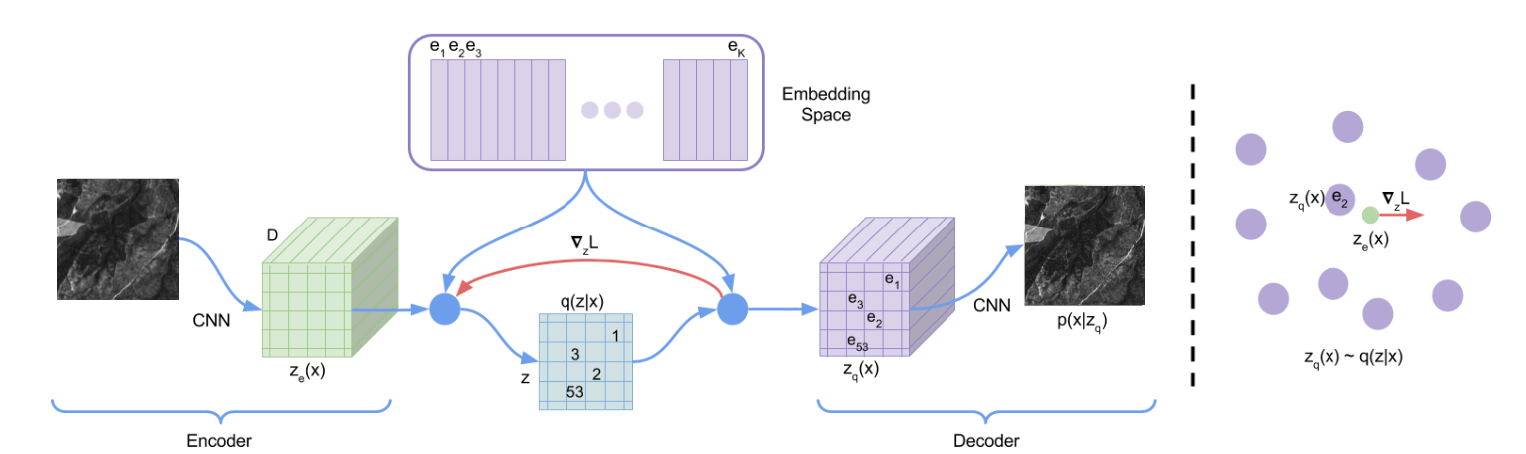
\includegraphics[width=\textwidth]{figures/VQVAE.png}
\caption{ Modified image from the original paper. The original image is encoded using an encoder. The encoded representation is 
then discretized using a learned codebook of vectors. Finally, to ensure successful decompression, we learned a decoder 
that can recover the original data.}
\label{fig-vqvae}
\end{figure}
 
\subsection{Encoder/Decoder:} 
When considering encoder-decoder pairs for temporal, spatial, and spatiotemporal data, the 
Convolutional Neural Network (CNN) emerges as a widely accepted choice. CNNs offer cost-
effectiveness and a pronounced ability to discern patterns. Notably, they cater to the intrinsic 
characteristic of such data types: translation equivariance. This means that when a CNN receives 
translated data, the output similarly reflects this translation. 
 
Quantization is the next phase, with a latent image as the foundational input. Here, the process occurs 
along the latent dimension, and each pixel in the latent space gets represented by a unique code. It’s 
essential to highlight that the latent image's resolution might not match the original. Often, this latent 
representation undergoes downscaling, enhancing the model's interpretative prowess regarding data 
relationships. The $dsf$(downscaling factor) determines the degree of this downscaling. Without 
downscaling (when $dsf$ = 1), quantization in the latent space resembles colour indexing, with each 
colour uniquely identified. In contrast, a larger $dsf$ allows for the indexing of broader data segments. 
 
Moving away from traditional max pooling, this method incorporates a convolutional neural network 
characterized by its stride. For clarity, a convolutional layer with a stride of 2, as it traverses the 
primary data, accounts for every other data point, leading to downscaling by a factor of 2. Significantly, 
each output pixel draws from a broader area than the $dsf$ might imply. This broader region, known 
as the “receptive field” in academic contexts, means that when downscaling is reversed during 
decoding, data accessed extends beyond just a single code. This ensures that even if a code undergoes 
modification, the change remains subtle and consistent with the dataset’s overall structure. This 
approach suggests a potential reduction in artifacts within the learned compression, a topic we will 
detail further in a subsequent section. To counteract potential data loss from downscaling, the latent 
space’s dimension is set larger than the original image’s, ensuring comprehensive data capture. 
 
Given an initial image with dimensions $W\times H\times B$  — where $W$  stands for width, $H$  represents 
height, and $B$  indicates channels—the encoded version takes on dimensions $\frac{W}{dsf}\times\frac{H}{dsf}\times D$. Here, $D$ 
signifies the latent space's dimension. While the original image spans a spatial surface of $WH$ , the 
encoded image covers $\frac{WH}{dsf^2}$.
 
\subsection{Quantization:} 
 
The quantization phase aims to transform a real vector into a discrete code, making it storage-ready. 
This transformation is inherently lossy. Central to quantization is clustering. Data points in the same 
cluster are denoted by an index and reconstructed from the cluster center. Information about the 
exact position within the cluster is what is typically lost during this step. Two dominant clustering 
approaches are in use: the traditional K-Means clustering and a gradient-based algorithm. The K-
Means method alternates between assigning data points to clusters and updating cluster centers. On 
the other hand, the gradient-based technique replaces the K-Means update rule with gradient 
descent. All cluster centers are collectively termed the codebook. As a result, the clustering algorithm 
outputs both the index of the assigned cluster and the value associated with a given data point. 
 
Considering the worst-case, the bit requirement ($b$) to store $\#C$ clusters is:
\begin{equation}
b = \lceil\log_2(\#C)\rceil
\end{equation}
For illustration:
\begin{itemize}
    \item With 1 cluster, 0 bits are sufficient since there's only one category. 
    \item 2 clusters necessitate 1 bit for differentiation (0 or 1). 
    \item 3 clusters require 2 bits for three possible categories (00, 01, or 10), leaving the 11 code 
unused.
    \item 4 clusters also demand 2 bits, using codes 00, 01, 10, and 11. 
\end{itemize} 
 
Expressing this in terms of $b$:
\begin{equation}
\#C=2^b
\end{equation}
% TODO add RVQ citation (soundstream)
This reveals that as $b$ bits of information are stored, the requisite cluster count escalates 
exponentially. This exponential growth directly influences memory usage during clustering. To 
counteract this exponential growth, Residual Vector Quantization (RVQ) was introduced. RVQ 
curtails the complexity from exponential to linear relative to the codebook size by employing multiple 
codebooks. For instance, with two codebooks and a vector $z$ to be quantized, the initial step quantizes 
$z$  to get cluster $z_0$ with index $c_0$ using the first codebook. Then, the residual $r = z -z_0$ is determined,
and the process is repeated, obtaining $z_1$ and $c_1$ from the second codebook. The final quantized vector 
and index are $z_0 + z_1$ and the concatenated $c_0$ and $c_1$, respectively. This method streamlines the 
complexity and memory demands of the quantization phase. The initial clustering sets a global 
position, whereas the subsequent clustering happens within the local cluster. Aggregation forms 
clusters, with an assumption of consistent structures within. Given $\#C_l$ as the cluster count per level, 
the total cluster count $\#C$ after $N$ layers is:
\begin{equation}
\#C=\#C_l^N
\end{equation} 
This equation can determine the clusters per level ($\#C_l$) required for a desired bit count b, as: 
\begin{equation}
\#C_l=2^{\frac{b}{N}}
\end{equation}
An enhancement to RVQ is the integration of a variable codebook count. During training, for each 
sample, the number of codebooks (N) is chosen randomly within a predefined range. This adaptive 
approach ensures model versatility to various codebook counts. 
 
A standout advantage of variable codebook counts is adaptability, allowing the application of a single 
model across different codebook quantities. For EO4EU, this adaptability is essential, reducing the 
models to be trained for distinct compression rates. Experiments presented in the subsequent section 
will demonstrate that this versatility has a minimal impact on model quality. 

\subsection{Lossless compression:} 
 
The concluding compression phase uses a standard lossless encoding algorithm on the cluster index 
numbers. As posited by Shannon's source coding theorem, the efficacy of an ideal lossless 
compression algorithm can be bounded by the entropy derived from the probability distribution of 
the cluster indexes. The calculations from the prior sections present a worst-case scenario, which is 
most pertinent in situations where the data is uniformly random, leading to maximized entropy. 
Subsequently, in the evaluation section, we adhere to standard practices in the literature, noting the 
theoretical compression ratio. This is especially relevant considering that multiple optimal algorithms 
can achieve this ratio when the index distribution is well-defined. 

%TODO check SSL description on data.
\section{Data type selection and data preparation}
Much like the discussions in Section 2.2.2 on data type selection for SSL models, for learned 
compression we chose Sentinel-2 multispectral images as our guiding data. We leveraged the auxiliary 
code blocks developed for SSL. Unlike SSL where parts of the data were removed, we preserved all 
data. In a compression context, factors such as high cloud coverage of satellite images do not 
compromise the task accuracy. The aim is to faithfully reconstruct the original image, independent of 
its content. Otherwise, the data preparation mirrors the SSL approach, as detailed in Section 2.2.2. 
The training dataset comprises roughly 413k samples, while the test set contains about 88k samples. 
 
When it comes to the training and development of learnt compression models on other data sources 
the setting is in a sense even simpler than the one in SSL. One needs to only adjust the input layers to 
the input data structures and obviously there are no augmentations to consider. We will provide 
compression models for at least one more data source used in the use cases. We see a considerable 
opportunity, as well as challenge, for learned compression on ECMWF CAMS datasets which have a 
three-dimensional, instead of two-dimensional structure.  We can practically adopt the same 
approach as in the Sentinel-2 case where we simply replace the 2D convolutions over the input data 
with 3D convolutions. ECMWF has published a nature paper where they release a full resolution 
dataset without internal compression33. The CAMS dataset34 presented in the paper is 153 MB for 1 
level and 21 GB for the 137 levels for the whole world on 109 variables. 
 
Having a model architecture that treats both 2D and 3D data should enable the treatment of the 
majority of grid like data structures. For example, ERA5 Land has the same structure as Sentinel 2 data 
and our model can be retrained to support these data sources. 
\section{Model Evaluation protocol} 
 
In evaluating learned compression models, the challenges differ from those in a supervised approach. 
In the latter, a single performance metric can be sufficient to compare different models. However, for 
learned compression, there's a need to balance two essential objectives: the degree of compression 
and the accuracy of the reconstructed output. A compression model is said to Pareto dominate 
another if it excels in both these criteria. In cases where no model has clear Pareto dominance, the 
choice becomes subjective, influenced by the specific problem, its demands, and the preferences of 
the researcher or designer. Our goal is to juxtapose our solutions with a relevant baseline, thereby 
highlighting the interplay between compression and fidelity. 
 
% 33 Klöwer, M., Razinger, M., Dominguez, J.J. et al. Compressing atmospheric data into its real 
% information content. Nat Comput Sci 1, 713–724 (2021). https://doi.org/10.1038/s43588-021-
% 00156-2 
% 34 CAMS Forecast Experiment using GRIB IEEE Data Encoding (CAMS, 2021); 
% https://doi.org/10.21957/56GH-9Y86 
 
To visualize this trade-off, we plot it on a two-dimensional graph. This representation provides a 
straightforward understanding of the tension between compression level and reconstruction 
accuracy. As a benchmark, we use the JPEG algorithm, interpreting the images from each band as 
monochromatic, single-channel visuals. To traverse this landscape of trade-offs, we select diverse 
compression ratios, noting the corresponding fidelity (quantified by compression error) alongside. 
 
The compression degree is gauged using the metric "bit per pixel" ($bpp$). This metric is derived by 
dividing the total byte size of the image by its pixel count. For JPEG, we consider the file size. For 
learned compression, we opt for entropy to ensure our metrics aren't influenced by the choice of 
lossless compressor. 
 
The maximal compression ratio for learned compression is found by determining the bits needed to 
represent a single code, based on the number of clusters per layer ($\#C_l$) and the layer count ($N$):
\begin{equation}
b = \lceil N \log_2(\#C_l)\rceil
\end{equation}
The entire code count is:
\begin{equation}
\frac{WH}{dsf^2}
\end{equation}
Subsequently, the bit per pixel ($bpp$) is:
\begin{equation}
bpp=\frac{N\log_2(\#C_l)}{dsf^2}
\end{equation}
 
For measuring errors, we deploy the root mean square error (RMS) as a percentage. This error is 
normalized to ensure values range between $0\%$ and $100\%$.

\section{Model Training}

% Add citation of Magda and co
In our initial investigations, we utilized a variant of VQ-VAE, aiming to limit codebook usage to boost 
performance. However, early tests revealed a tendency for the model to prioritize reducing the 
codebook size, sometimes using only a few of its elements. This phenomenon, known as "degenerate 
outcomes," necessitated an adjustment. We briefly experimented with a modified regularizer, 
focusing solely on reconstruction error. This quickly underscored the scalability concerns that had 
originally led to the introduction of RVQ. 
 
During this phase, we also found Batch Normalization to be particularly batch size-sensitive, 
prompting its replacement with Layer Normalization. Furthermore, we settled on a down-sampling 
factor ($dsf$) of 2, striking a balance between memory efficiency and the risk of over-smoothing from 
excessive downscaling. 

% TODO add figure + ref.

Figure 7 visually depicts the encoder's intricate architecture, which is divided into three main 
segments: 
 
\paragraph{Optional Downscaling:} Situated at both the start and end of the architecture, this section uses 
convolution with a stride of 2 for downscaling when needed, and standard convolution otherwise. For 
instance, with a dsf of $2$, only the initial downscaling is activated; for a $dsf$ of 4, both are engaged. 
 
% 35 Gregorová, Magda, Marc Desaules, and Alexandros Kalousis. "Learned transform compression 
% with optimized entropy encoding." arXiv preprint arXiv:2104.03305 (2021). 

\paragraph{Convolutional Core:} This central segment boasts two main blocks, each housing three sub-blocks. 
These sub-blocks each consist of two convolutional layers, augmented by a ReLU non-linearity and 
layer normalization. This arrangement amasses a total of twelve convolutional layers throughout. 
Residual Connections: To bolster information retention and continuity, residual skip connections are 
introduced between each primary block at every hierarchical stage. This structural decision ensures 
that data is consistently maintained across the hierarchy, allowing the model to selectively infuse data 
when deemed essential. 

\begin{figure}
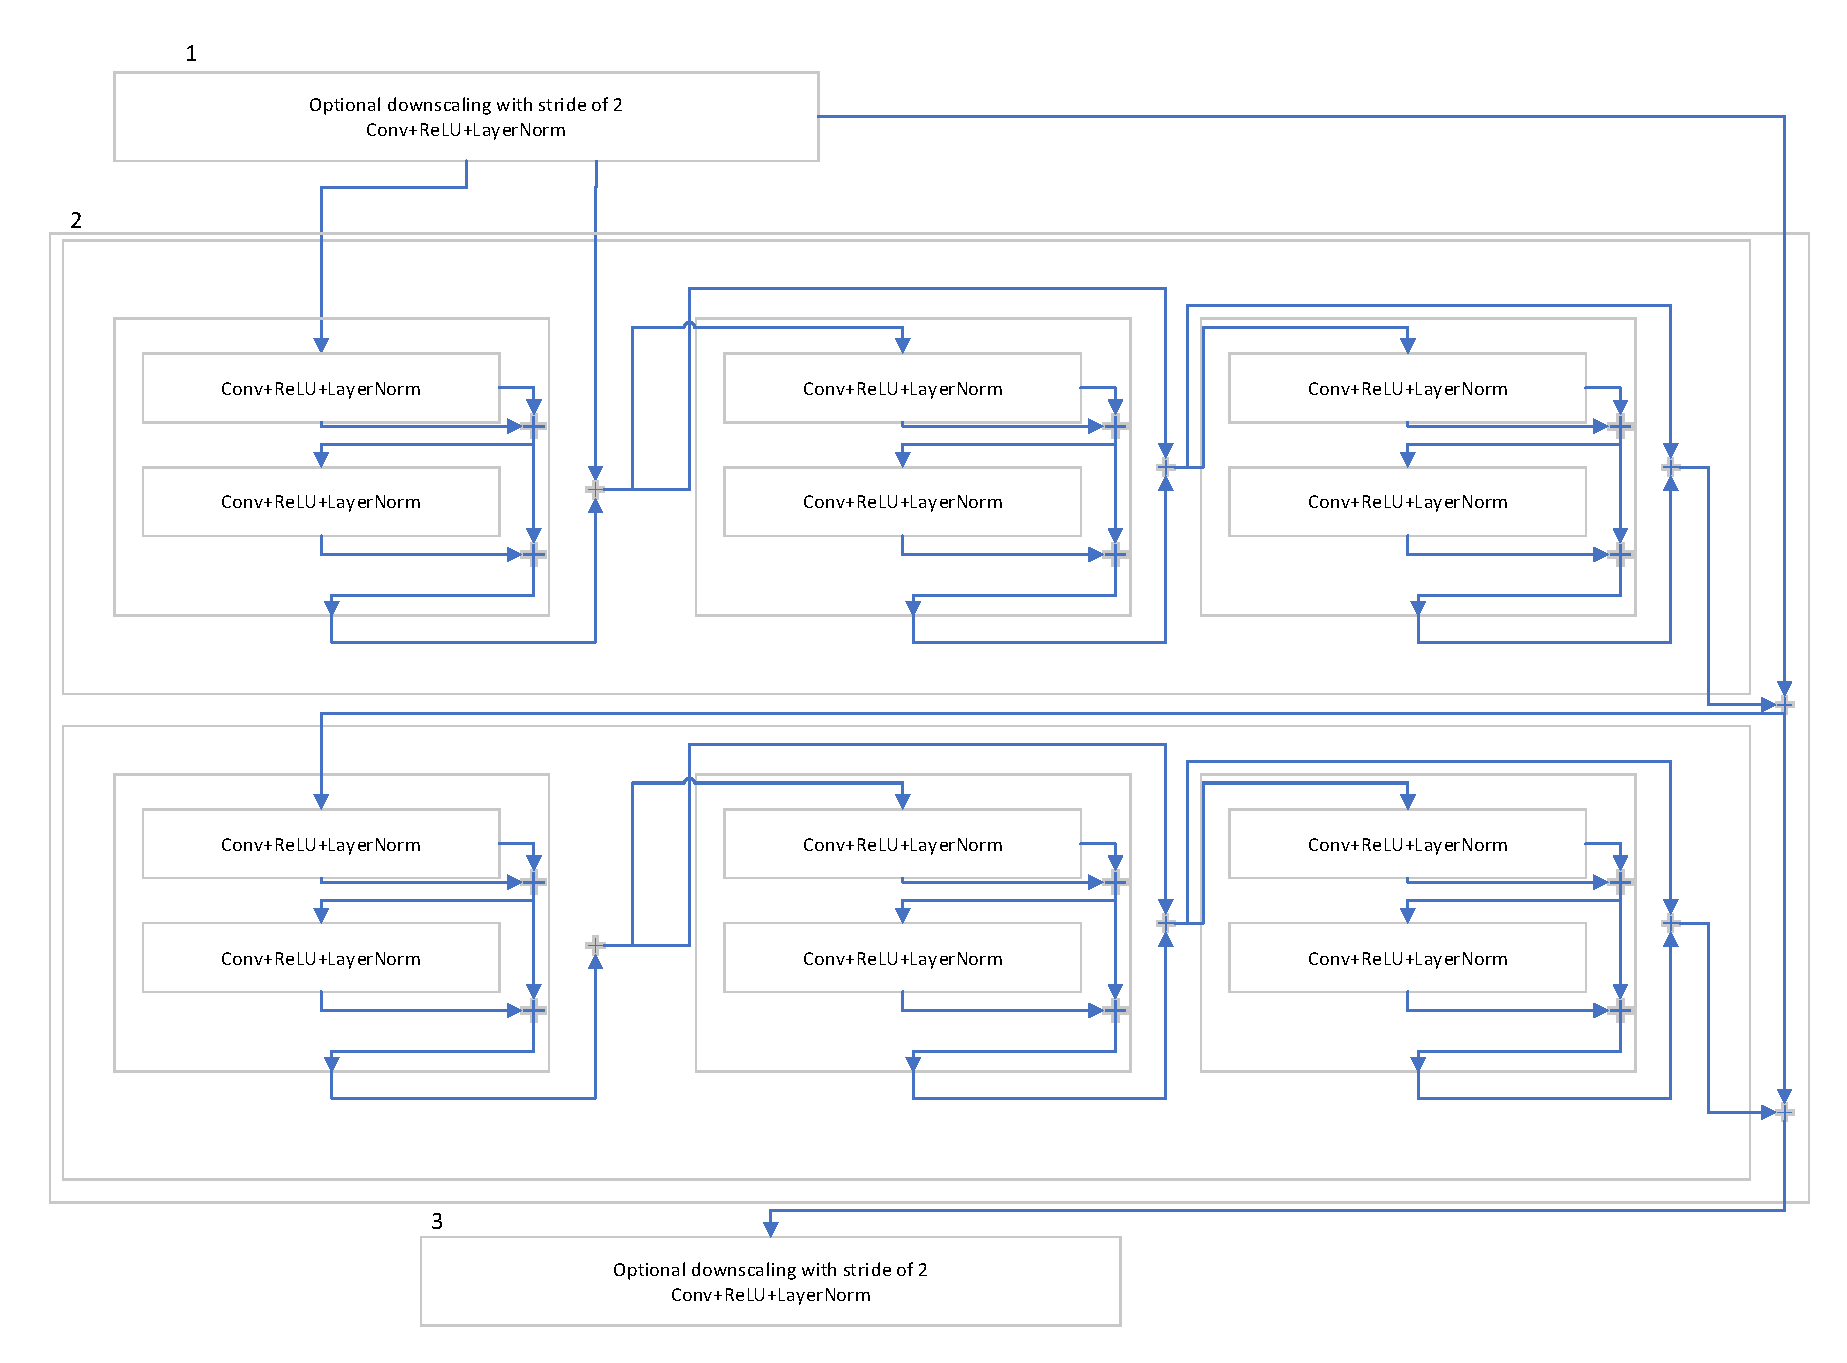
\includegraphics[width=\textwidth]{figures/ArchitectureCompression.pdf}
\caption{Encoder Architecture. The black numbers refer to the architecture description. The "+" node denotes addition operations. The blue arrows indicate data flow. The boxes denote component groupings.}
\end{figure} 
 
Decoding is relatively straightforward; we use a mirrored version of the encoder architecture. This 
symmetry involves transposed convolutions, effectively backtracking through the encoding steps to 
recreate the initial data. 
 
The models are trained using Adam optimizer with a fixed learning rate. 
 
During training, we encountered two primary challenges. First, GPU memory restrictions were a 
constraint. This was accentuated by the Sentinel data’s >10 channels—compared to the typical 3 in 
RGB images—and the use of expansive image patches. The second challenge stemmed from the sheer 
size of the dataset. This necessitated optimized I/O during training to ensure timely completion.

\section{Model finetuning and evaluation}
The key hyperparameters requiring fine-tuning include: 
\paragraph{Downscaling Factor ($dsf$):} Represented by the number of layers with a stride of 2, the $dsf$ determines 
the reduction level applied to the original image (1x, 2x, or 4x). It directly influences the dimensions 
of the spatial latent space and the size of a single latent code's receptive field. Intensified 
downsampling requires the model to encapsulate a larger spatial region within a single code, 
potentially leading to finer detail loss. Conversely, limited downsampling retains more details but 
compromises compression efficacy. Although we primarily employed a 2x factor, we also ventured 
into analyses with factors of 1x and 4x. 
\paragraph{Latent Space Channels:} The number of channels in the latent space is pivotal. Our selection aimed to 
strike a balance—choosing a figure substantial enough to avoid overfitting, considering our dataset's 
size, while also being mindful of memory constraints. We settled on 128 channels. Notably, this 
parameter doesn't have a direct bearing on compression. Hence, our detailed exploration was limited. 
Furthermore, to ensure that the latent space's size wasn't restrictive, we trained an autoencoder 
without quantization, confirming that the latent space wasn't a bottleneck. 
\paragraph{Codebook Configuration:} This involves the number of codebooks ($N$) and the size of each 
codebook($\#C_l$). Directly impacting the model's compression and quality, the effective codebook size 
is derived as $\#C_l^N$. Our typical configuration utilized codebooks of size 10,000 and incorporated up to 
8 codebooks. 
In essence, the primary determinants of compression are the $dsf$ and the codebook’s configuration—
both its size and quantity. Other parameters, while influential, are primarily constrained by GPU 
memory capacities, especially when handling large datasets, rather than influencing compression 
directly.

\begin{figure}
    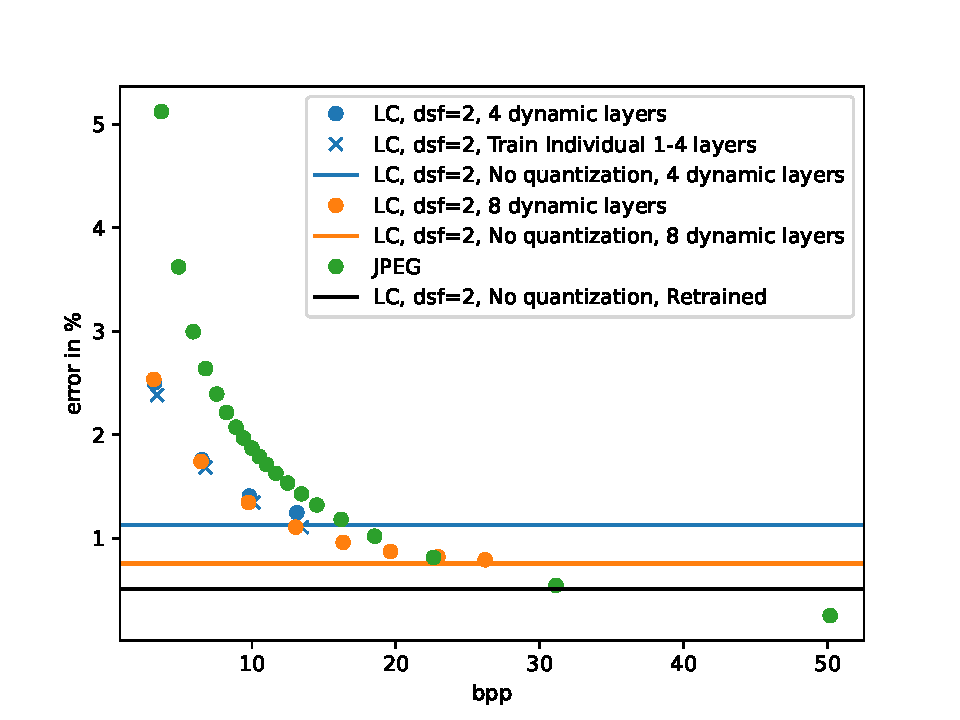
\includegraphics[width=\textwidth]{figures/loss.pdf}
    \caption{Reconstruction quality versus compression rate. 
On the x axis we show the compression rate expressed as bit per pixel, on the y axis we show the error expressed in 
percentage. Each dot consists of a trained model and its performance. Line represent performance of none-quantized 
models. Data raw bpp is 120.}
\label{fig-loss}
\end{figure}

%TODO figure and reference
The experiments conducted are visualized in Figure \ref{fig-loss}. The x-axis represents compression in $bpp$, while 
the y-axis displays the $RMS$ in percentage. Here's a breakdown of the conducted experiments: 
\begin{description}
\item[Dynamic Number of Codebooks (Blue Dots):] A model was trained using a dynamic range of 
codebooks, varying from 1 to 4, over the course of a week. The outcomes of this training are 
represented by blue dots on the graph.
\item[Fine-Tuning with Fixed Number of Codebooks (Blue Crosses):] Following the initial training, 
each of the 4 models was further fine-tuned, with a fixed number of codebooks, for an 
additional four days. These results are indicated by blue crosses in the figure. 
\item[Evaluation without Quantization (Continuous Blue Line):] The performance of the model, 
when evaluated without quantization, is depicted as a continuous blue line on the graph.
\item[Continuous Model without Quantization (Black Line):] A continuous model, devoid of 
quantization, was trained over a span of 4 days. It leveraged weights from the preceding 
dynamic model. The resultant performance is shown as a black line, serving as a reference 
point or lower bound for the given training time and network architecture.
\item[Eight Dynamic Number of Codebooks (Orange Dots):] A model was trained over four days with 
eight dynamic codebooks. This model was initialized using the weights from the earlier 
continuous solution. The outcomes of this model are symbolized by orange dots on the figure.
\item[Evaluation of the 8-Codebook Model without Quantization (Continuous Orange Line):] The 
same model, when assessed without quantization, is represented by a continuous orange line 
on the chart.
\item[JPEG Performance:] The efficiency of the JPEG standard was also assessed by modulating the 
quality parameter in the compression. 
\end{description}
 
The results of these various experiments offer insights into the capabilities and potential 
enhancements of the models, as well as a comparative analysis with traditional compression methods 
like JPEG.
Based on the conducted experiments and the data visualized in Figure \ref{fig-loss}, the following conclusions 
can be drawn: 

\begin{itemize}
    \item Efficacy of Dynamic Number of Codebooks: The use of a dynamic number of codebooks 
seems to be effective with a marginal performance cost. This is evident from the proximity of 
results between models depicted by the blue dot (dynamic codebook model) and blue cross 
(fine-tuned fixed codebook model). 
\item Performance of Autoencoders Without Quantization: For models trained with quantization, 
the autoencoder's performance without quantization tends to align with the performance 
achieved using the highest number of codebooks during training.
\item Potential for Autoencoder Performance: The autoencoder's potential hasn't been fully 
tapped, as suggested by the superior performance of the model trained without quantization 
(represented by the black line).
\item Saturation of Performance Improvement: As the $bpp$ escalates, the performance 
enhancement of the model plateaus post-20 $bpp$. It's speculated that this stems from the 
inherent limitations of the learned compression algorithm. When trained for a constrained 
period using a finite dataset, the algorithm possesses intrinsic errors. In comparison, 
traditional algorithms like JPEG, when set to maximum quality, are mathematically designed 
to retrieve the original data, whereas the machine learning counterparts aren't.
\item Model Accuracy: A significant majority of the models tested showcased errors below the 2\textbackslash{}% 
threshold.
\end{itemize}

\begin{figure}
\begin{minipage}{0.27\linewidth}
    \tiny
    Original\\
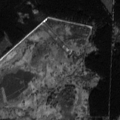
\includegraphics[width=1\linewidth]{figures/compression/original.png}
\end{minipage}
\tiny
\begin{tabular}{ccc}
   LC   & \begin{minipage}{0.27\linewidth}\tiny$n=1$\\$\textbf{bpp}=3.2$ ($2.4 \%$)\\ 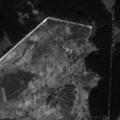
\includegraphics[width=\linewidth]{figures/compression/reconstruction2.png}   \end{minipage}%
   &  \\ \\
   JPEG   & \begin{minipage}{0.27\linewidth}\tiny quality$=5$\\$\textbf{bpp}=3.7$ ($5.1 \%$)\\ 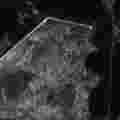
\includegraphics[width=1\linewidth]{figures/compression/reconstructionJPEG5.png}\end{minipage} &%
\begin{minipage}{0.27\linewidth}quality$=20$\\$\textbf{bpp}=6.8$ ($2.6 \%$)\\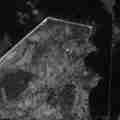
\includegraphics[width=1\linewidth]{figures/compression/reconstructionJPEG20.png}\end{minipage}%
\end{tabular}
\caption{Visual comparison of a single instance of the first band between the learned compression model with a single 
quantization layer and JPEG. The first JPEG image has similar bpp whereas the second JPEG image has similar error.}
\label{fig-comp1}
\end{figure}

% \begin{figure}
% \begin{minipage}{0.27\linewidth}
%     \tiny
%     Original\\
% 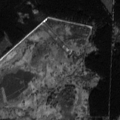
\includegraphics[width=1\linewidth]{figures/compression/original.png}
% \end{minipage}
% \tiny
% \begin{tabular}{ccc}
%    LC   & \begin{minipage}{0.27\linewidth}\tiny$n=2$\\$\textbf{bpp}=6.5$ ($1.8 \%$)\\ 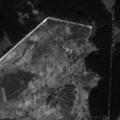
\includegraphics[width=\linewidth]{figures/compression/reconstruction2.png}   \end{minipage}%
%    &  \\ \\
%    JPEG   & \begin{minipage}{0.27\linewidth}\tiny quality$=20$\\$\textbf{bpp}=6.8$ ($2.6 \%$)\\ 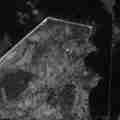
\includegraphics[width=1\linewidth]{figures/compression/reconstructionJPEG20.png}\end{minipage} &%
% \begin{minipage}{0.27\linewidth}quality$=50$\\$\textbf{bpp}=10.5$ ($1.8 \%$)\\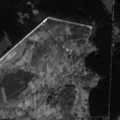
\includegraphics[width=1\linewidth]{figures/compression/reconstructionJPEG50.png}\end{minipage}%
% \end{tabular}
% \caption{Visual comparison of a single instance of the first band between the learned compression model with two 
% quantization layer and JPEG. The first JPEG image has similar bpp whereas the second JPEG image has similar error}
% \label{fig-comp2}
% \end{figure}

% \begin{figure}
% \begin{minipage}{0.27\linewidth}
%     \tiny
%     Original\\
% 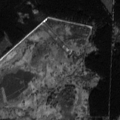
\includegraphics[width=1\linewidth]{figures/compression/original.png}
% \end{minipage}
% \tiny
% \begin{tabular}{ccc}
%    LC   & \begin{minipage}{0.27\linewidth}\tiny$n=3$\\$\textbf{bpp}=9.8$ ($1.4 \%$)\\ 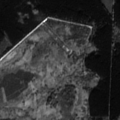
\includegraphics[width=\linewidth]{figures/compression/reconstruction3.png}   \end{minipage}%
%    &  \\ \\
%    JPEG   & \begin{minipage}{0.27\linewidth}\tiny quality$=40$\\$\textbf{bpp}=9.4$ ($2 \%$)\\ 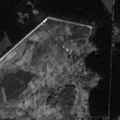
\includegraphics[width=1\linewidth]{figures/compression/reconstructionJPEG40.png}\end{minipage} &%
% \begin{minipage}{0.27\linewidth}quality$=70$\\$\textbf{bpp}=13.5$ ($1.4 \%$)\\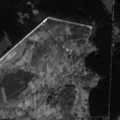
\includegraphics[width=1\linewidth]{figures/compression/reconstructionJPEG70.png}\end{minipage}%
% \end{tabular}
% \caption{Visual comparison of a single instance of the first band between the learned compression model with two 
% quantization layer and JPEG. The first JPEG image has similar bpp whereas the second JPEG image has similar error}
% \label{fig-comp3}
% \end{figure}

\begin{figure}
\begin{minipage}{0.27\linewidth}
    \tiny
    Original\\
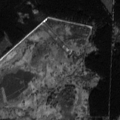
\includegraphics[width=1\linewidth]{figures/compression/original.png}
\end{minipage}
\tiny
\begin{tabular}{ccc}
   LC   & \begin{minipage}{0.27\linewidth}\tiny$n=4$\\$\textbf{bpp}=13.1$ ($1.2 \%$)\\ 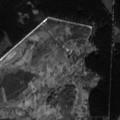
\includegraphics[width=\linewidth]{figures/compression/reconstruction4.png}   \end{minipage}%
   &  \\ \\
   JPEG   & \begin{minipage}{0.27\linewidth}quality$=70$\\$\textbf{bpp}=13.5$ ($1.4 \%$)\\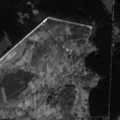
\includegraphics[width=1\linewidth]{figures/compression/reconstructionJPEG70.png}\end{minipage}&%
\begin{minipage}{0.27\linewidth}quality$=80$\\$\textbf{bpp}=16.2$ ($1.2 \%$)\\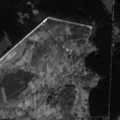
\includegraphics[width=1\linewidth]{figures/compression/reconstructionJPEG80.png}\end{minipage}%
\end{tabular}
\caption{Visual comparison of a single instance of the first band between the learned compression model with two 
quantization layer and JPEG. The first JPEG image has similar bpp whereas the second JPEG image has similar error}
\label{fig-comp4}
\end{figure}

The purely quantitative assessments, though informative, offer only a partial understanding of the 
overall performance. A qualitative examination of visual quality provides another layer of insight, as 
evidenced when comparing images compressed using JPEG and learned compression methods. 

%TODO: Figure
Figure \ref{fig-comp1} through \ref{fig-comp4} display this comparison, focusing on the use of 1 to 4 layers of quantization. A 
noticeable characteristic of JPEG compression is the presence of blocking artifacts; these manifest as 
8 by 8 pixel blocks which directly correspond to the block size utilized by the JPEG algorithm. In stark 
contrast, images compressed via the learned method are devoid of such artifacts. 
 
This superior visual consistency in learned compression is likely attributable to its holistic approach to 
image compression. Rather than segmenting and processing the image in discrete blocks, the learned 
compression processes the entire image as an integrated entity. This method ensures smooth 
transitions and consistent patterns across neighboring pixels, eliminating the blocking artifacts that 
are evident in JPEG. 
 
This research demonstrates the efficacy of learned compression techniques. Not only do these 
methods achieve efficient image compression, but they also preserve the perceptual quality of 
images, making them a competitive alternative to traditional methods like JPEG in terms of 
compression and visual fidelity.

\section{Quantifying the effect of compression with respect to downstream tasks:} 

To assess the impact of compression on machine learning tasks, we evaluated the binary cross-entropy 
error of a baseline classifier when applied to compressed versus original data. We employed T-tests 
to compare the error rates of compressed versus original data to determine if the compression 
resulted in a significantly different error. Our findings indicate that there is no substantial difference 
in error across all models, with the exception of the lowest compression setting, which utilizes only 
one out of eight codebooks. Interestingly, in this setting, the compressed data yielded a slightly better 
result, reflected in a p-value of 0.02. However, considering the marginal nature of this improvement 
and the higher p-values observed in other settings, the results do not appear to be significant. 
 
We also computed the symmetric KL divergence for every instance for each label individually and 
created their histogram. The histogram follows a distribution with a very long tail, with the majority 
of the probability mass near 0. This is visualized in Figure 13. 
Finally, to quantify the effect on class assignment, we categorized the label into four categories: Surely 
No, Maybe No, Maybe Yes, Surely Yes, with boundaries at probabilities of 25\%, 50\%, and 75\%. We 
created the contingency matrix of these categories and found that, as expected, the majority are near 
the diagonal. This shows that there are only a few changes in classification due to compression. We 
visualize one of these results in Figure 14. 

\begin{figure}
\begin{minipage}{0.45\linewidth}
1/8:\\
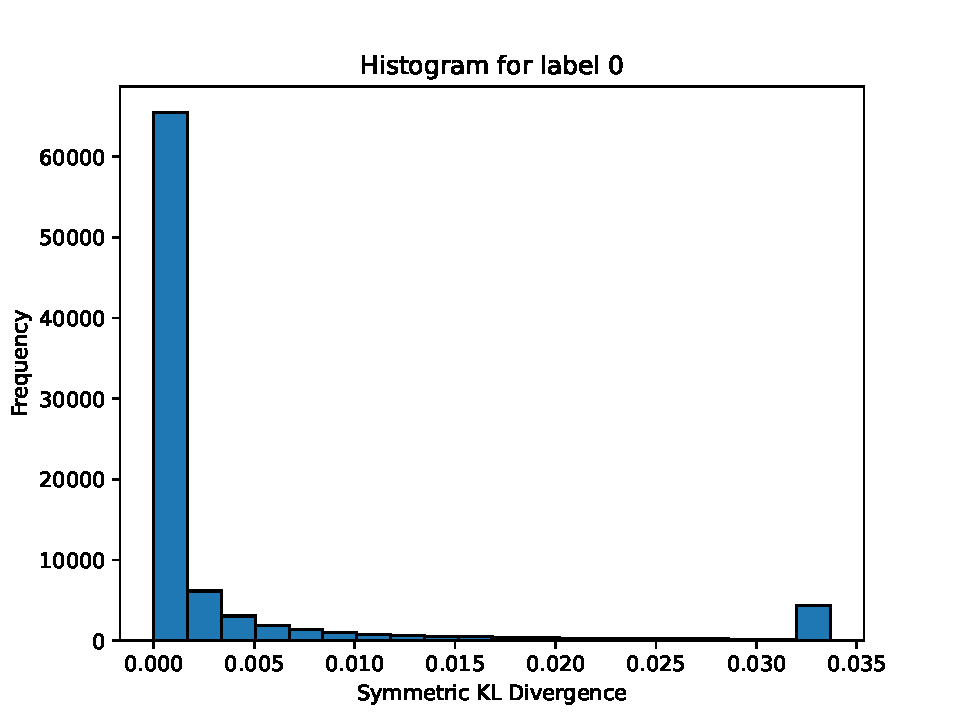
\includegraphics[width=1.2\textwidth,trim= 0 0 0 0.9cm,clip]{figures/8_1_histogram_0.pdf}
\end{minipage}
\hfill
\begin{minipage}{0.45\linewidth}
    8/8:\\
    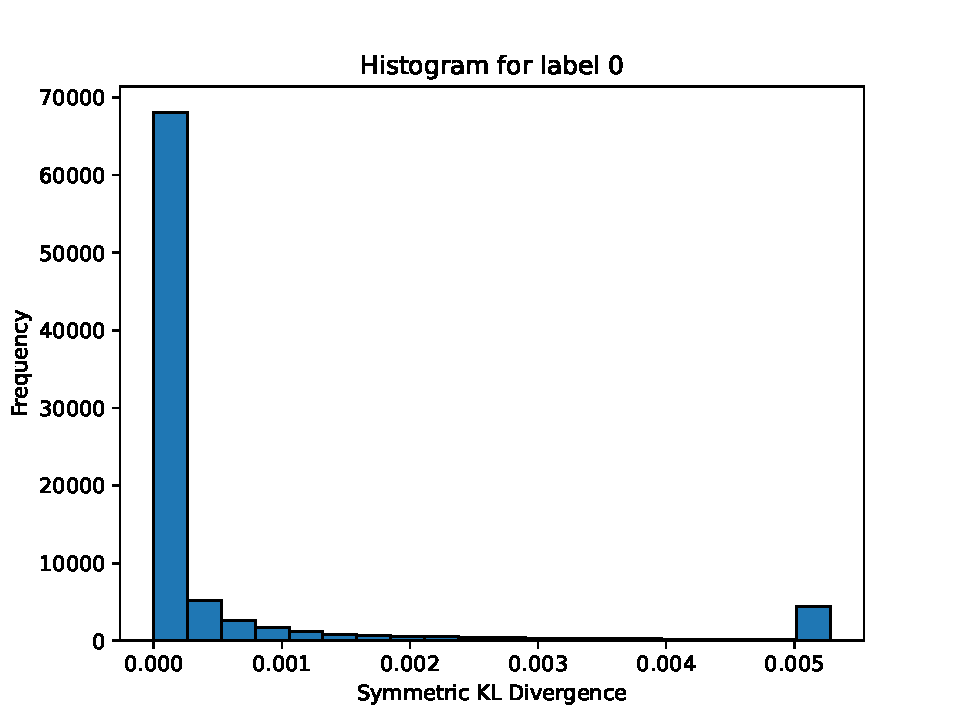
\includegraphics[width=1.2\textwidth,trim= 0 0 0 0.9cm,clip]{figures/8_8_histogram_0.pdf}
\end{minipage}
\caption{Histogram of the first label of the Symmetric KL Divergence of the most compressed model. The last bin is 
unbounded and contain 5 percents of the data.}
\end{figure}

\begin{figure}
\begin{minipage}{0.5\linewidth}
1/8:\\
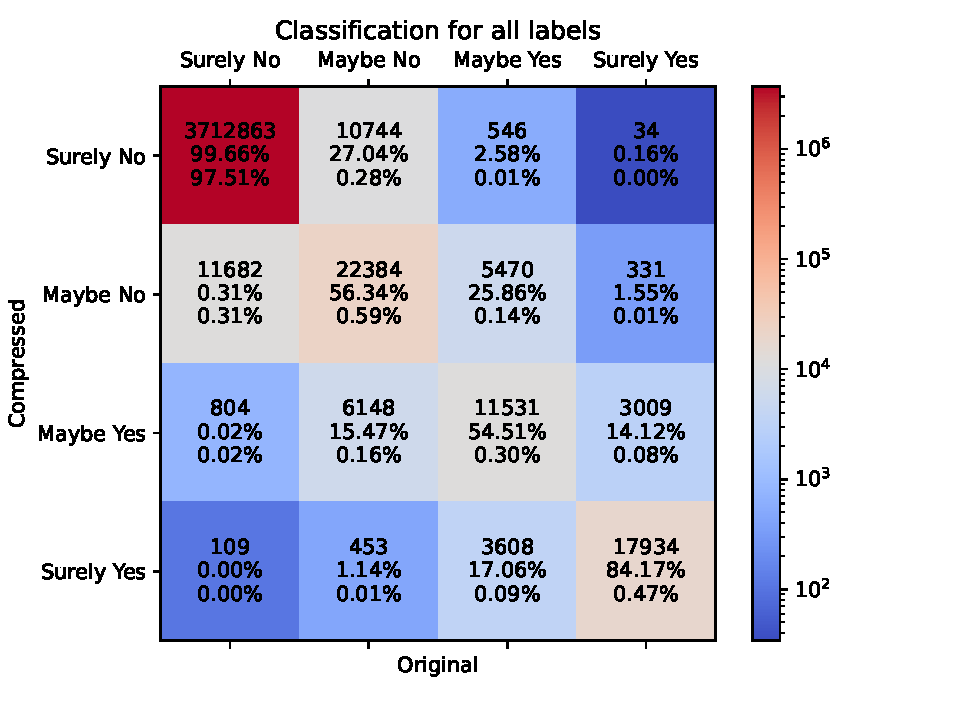
\includegraphics[width=1.1\textwidth,trim= 0 0 0 0.9cm,clip]{figures/8_1_contengency_combined.pdf}
\end{minipage}
\hfill
\begin{minipage}{0.5\linewidth}
8/8:\\
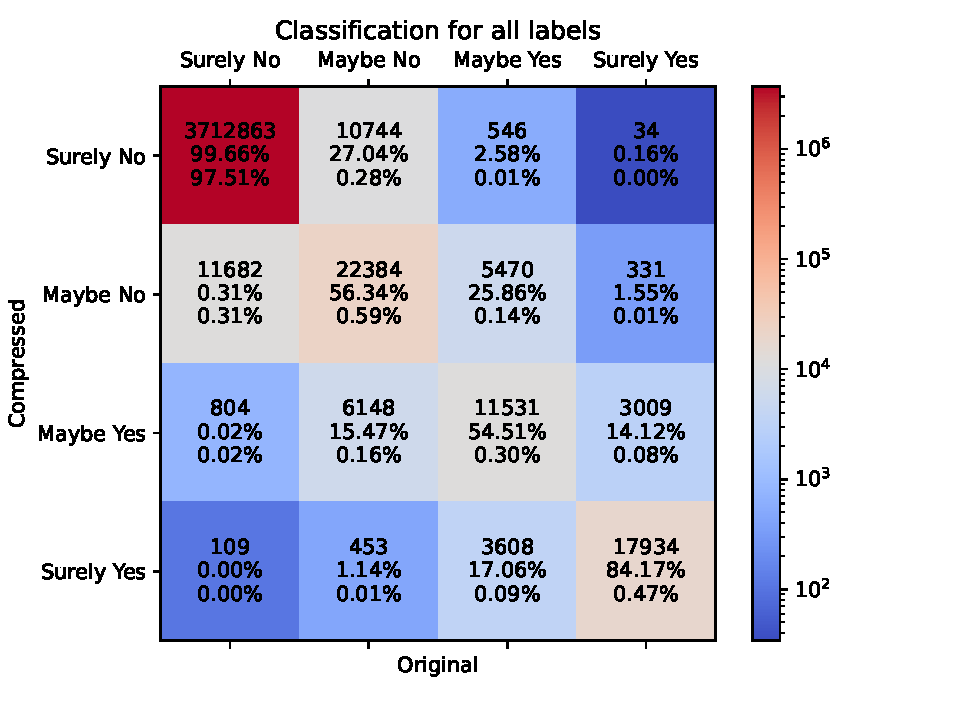
\includegraphics[width=1.1\textwidth,trim= 0 0 0 0.9cm,clip]{figures/8_1_contengency_combined.pdf}
\end{minipage}
\caption{Contingency matrix for all labels showing the miss classification due to compression. This is done here with 
the most compressed model (using only 1 of the 8 codebooks).}
\end{figure}

\printbibliography

\end{document}
